% The 12pt option is required by the 2001/02 thesis regulations
% Hacked together from the LaTeX template from the maths department of UoM


%This is just the standard line that tells the virtual "printer" what document we're making.
% Remove the twoside option for single-sided printing
\documentclass[12pt,PhD,twoside]{muthesis}

%These are the citation styles.
\usepackage[backend=bibtex,style=nature,citestyle=nature]{biblatex} %science, nature, alphabetic are common choices.
%FYI
% Citations styles = https://www.sharelatex.com/learn/Biblatex_citation_styles
% Bibliography styles = https://www.sharelatex.com/learn/Biblatex_bibliography_styles


\usepackage{graphicx} %use [!ht] (which means ignore sensible protocols and place here) not [h] (which means place here-ish) for figures otherwise they end up at the end of the chapter.

\usepackage{amsmath}
\usepackage{csquotes}
\usepackage{longtable}
\usepackage[acronym]{glossaries} %Whilst it's tempting, I've found tinkering with glossary structure and style is a nightmare. Avoid at all costs.
\addbibresource{references.bib} % This is the folder containing all your "bibtex" references. All reference managers can export to this format.
\graphicspath{{images/}} %Store all your figures here

% abbreviations: The first option in the curly braces is the code used in the text, second is the short form, and third is the long form. http://tex.stackexchange.com/questions/86666/how-to-create-both-list-of-abbreviations-and-list-of-nomenclature-using-nomencl
\newacronym{pm}{PM}{Plasma Membrane}
\newacronym{md}{MD}{Molecular Dynamics}
\newacronym{tm}{TM}{Transmembrane}
\newacronym{tmh}{TMH}{Transmembrane Helix}
\newacronym{tmp}{TMP}{Transmembrane Protein}
\newacronym{er}{ER}{Endoplasmic Reticulum}
\newacronym{ta}{TA}{Tail Anchor}
\newacronym{pdb}{PDB}{Protein Data Bank}
\newacronym{snare}{SNARE}{Soluble N-Ethylmaleimide-Sensitive Factor Attachment Receptor}

% nomenclature:
%\newglossaryentry{angelsperarea}{
  %name = $a$ ,
%  description = The number of angels per unit area,
%}

\makeglossaries

\begin{document}
\title{Investigating the Recognition and Interactions of Non-Polar $\alpha$ Helices in Biology}
\author{James Baker}
\faculty{Life Sciences}
\def\wordcount{xxxxx}

% Uncomment the line below to suppress the `List of Tables' page (optional)
\tablespagefalse

% Uncomment the line below to suppress the `List of Figures' page (optional)
\figurespagefalse

% Uncomment the line below to use a customised Declaration statement
%\def\declaration{All the work in this thesis has been sourced from Google}

\beforeabstract % Don't move the abstract, it doesn't like it.
Transmembrane $\alpha$ helix containing proteins make up around a quarter of all proteins, as well as two thirds of drug targets, and contain some of the most critical proteins required for life as we know it. Yet they are fundamentally difficult to study experimentally. This is in part due to the very features that make them so biologically influential: their hydrophobic transmembrane helices. What is missing in the current literature is a nuanced understanding of the complexities of the helix composition beyond a hydrophobic region of around 20 residues. Currently it is known that the properties of transmembrane protein $\alpha$ helices underpin membrane protein insertion mechanisms and furthermore can be used to predict presence of function in the transmembrane helix itself. By leveraging large datasets of transmembrane proteins, this thesis is focussed on characterising features of $\alpha$ helices en masse, particularly regarding their topology, membrane-protein interactions, and intra-membrane protein interactions.

Herein we expand on the core understanding of the biophysicochemical properties of these helices. We find evidence of a universal ``negative-not-inside'' rule that complements the famous ``positive-inside rule'' as well as intramembrane leucine propensity for the inner leaflet.

Furthermore we provide an up-to-date dataset of potential Tail-Anchored proteins, a group of post-translationally inserted proteins.
\afterabstract


%The preface section doesn't like being in a different document for some reason. (I think it's just my compiler, there is no reason why it shouldn't work)
\prefacesection{Acknowledgements}
Together my supervisory team have instilled in me an excitement of discovery. Furthermore they have taught me a deep value of inductive reasoning and inference over deduction.

Shout out to all the Biopython devs that saved my sanity!

\subsection*{Preamble} %A side note. the "*" hides the section number.
In the 1950s and 1960s, the field of biological philosophy was still emerging. David Hull writes on the matter in his 1969 entitled {\it``What Philosophy of Biology is not''}:

\begin{displayquote}
``Periodically through the history of biology, biologists have tried to do
a little philosophy...'' \cite{Hull1969}
\end{displayquote}

I think this accurately summarises my attempts at applying philosophy to science for my philosophical doctorate. I can't help but wish my thesis title was ``The ins-and-outs of greasy peptides''.

So long, and thanks for all the fish!

\prefacesection{List of publications}

\subsection*{Journal Articles} % the * hides the section number

\subsection*{Posters}
Baker, J. and Warwicker, J. A Bioinformatic Method to Identify Potential SNARE Proteins. {\it 40th FEBS Congress} Late Breaker (2015)

\afterpreface % DO NOT DELETE. BAD THINGS HAPPEN.

%This is where we call the chapters. No need to include ".tex" The chapters will be printed to the document in this order.
\chapter{Introduction}

\section{On The Importance of Membranes}
%to do:  give specific examples of incredibly useful membrane protiens. Outline that MPs are vital for relaying information and chemistry across the membrane.
When looking at the title of this thesis one might be surprised to first be reading not about protein helices, but membrane lipids. However, it is critical to understand that the two are inextricably linked, and often what we observe from the $\alpha$ helices reflect the properties of the much harder to study membranes. The lipid membranes influence the local structure, dynamics, and activity of proteins in the membrane in non-trivial ways \cite{Bondar2010, Bondar2009, Jardon-Valadez2010, Kalvodova2005, Urban2005}. It has been known for some time that the outer membranes of Gram negative bacteria are asymentric in terms of lipid composition. The outer membranes contain lipopolysccharide, whilst the inner is a mixture of approximately 25 phospholipid types. Adding to the membrane asymmetry composition story, a thorough analysis of residue composition in yeast and human \gls{tmh} regions revealed intra-membrane leaflet composition asymetry in the \gls{er}, but not the Golgi \cite{Sharpe2010}. Furthermore protein\-lipid interactions have been shown to be determinants of membrane curvature \cite{Jensen2004}, and have complex biochemical solutions to hydrophobic mismatch \cite{Planque2003}. %the planque reference is messed up. It may need changing with every bib.tex update unless the permannet record is changed.

Membrane bound proteins underpin almost every biological process directly, or indirectly, from photosynthesis to respiration. Integral \gls{tmp} are encoded by around 30\% of the genes in the human genome which reflects their biological importance \cite{Almen2009}. These proteins allow biochemical pathways that traverse the various biological membranes used in life. The compartmentalisation of cellular biochemistry is arguably one of the most significant events to have occurred in evolution, and is certainly one of the fundamental prerequisites for life \cite{Koshland2002}. The proteins that allow life to use this biochemical barrier are perhaps equally important. However we must understand both the membranes and the proteins to get an accurate model of how this complex biological system functions.

\subsection{The History of Biological Membranes in Science}

More recently, the insertion and formation of the unusually orientated \gls{tmh}s and of the more traditional \gls{tmh}s have been shown to be underpinned by complex thermodynamic equilibria \cite{Cymer2014}. \gls{tmh}s have been identified as regulators of protein quality control and trafficking mechanisms, shifting the idea away from \gls{tmh}s broadly simply functioning as anchors \cite{Hessa2011}. The story is not as simple as originally thought. There is a contingency in the field of biological membranes that despite progress over the last decade, there is a lack of information regarding their structure, assembly, and the behaviour of \gls{tmh}s in the lipid bilayer; the native biological environment of \gls{tmh}s \cite{Ladokhin2015, Cymer2014}.

\subsection{Biological Membrane Composition}

%Something about aysmetry, varies through the tree of life. "before we discuss the membrane proteins, one must consider the biological reason as for why they exist."

There is a rich variety of lipid molecules that make up the biological membranes. Generally speaking, these lipids have a polar headgroup§, and a hydrophobic hydrocarbon ``tail''. Water entropicly drives the self association of the lipid molecules. In other words the bilayer forms from these phospholipid molecules due to the fierce dissociation between the polar water and the hydrophobic tails. This can be seen even in relatively early \gls{md} simulations \cite{Goetz1998}.

The majority of lipids in the membrane are phospholipids. These are composed of a glycerol molecule. Bonded to the glycerol molecule are two hydrophobic fatty acid tail groups, and a negatively-charged polar phosphate group. The polar phosphate group is modeified with an alcohol group.


\section{$\alpha$ Helices in Membranes }
\subsection{Transmembrane Helix Sequence Composition}

%This should basically be a summary of Pogozheva, Baeza-delgado, and  Sharpe. Cite examples of direct and indirect accurate prediction methods

%Wong papers on how the sequences contain nuanced signals.

%Function is a result of structure, and here the structure and sequence are supposedly very relatable.
The relationship between the membrane and \gls{tmp}s is underpinned by complex thermondynamic and electrostatic equilibria. Once inserted the protein doesn't leave the membrane as a result of the transmembrane helix being very hydrophobic. This hydrophobicity, and the hydrophobicity of the lipid tails means that they self associate. A better way of describing it is that they fiercely dissociate from the water. The overall $\Delta$G for a transmembrane helix in the membrane is -12kcal mol−1 \cite{Cymer2014}: the association of the helix in the membrane is typically spontaneous.

Because of the experimental hinderence, the story of transmembrane proteins has been relatively slow to emerge. In the 1990s and early 2000s the story was seemingly uncomplicated. There were membrane-spanning bundles of non-polar α-helices of roughly 20 residues length, with a consistent orientation of being perpendicular to the membrane surface. Since the mid-2000s the elucidation of many more intramembrane helix structures implied a far richer variety of transmembrane helices existed than previously thought, with a range of orientations and intra-membrane biophysical variations. Although the simple helices are broadly prevelant, hundreds of high quality membrane structures have elucidated that \gls{tmh}s can adopt a plethora of lengths and orientations within the membrane. \gls{tmh}s are capable of partial spanning of the membrane, spanning using oblique angles, and even lying flat on the membrane surface \cite{VonHeijne2006, Elofsson2007} (Figure \ref{fig:helixcartoon1}).

\begin{figure}[!ht]
\centering
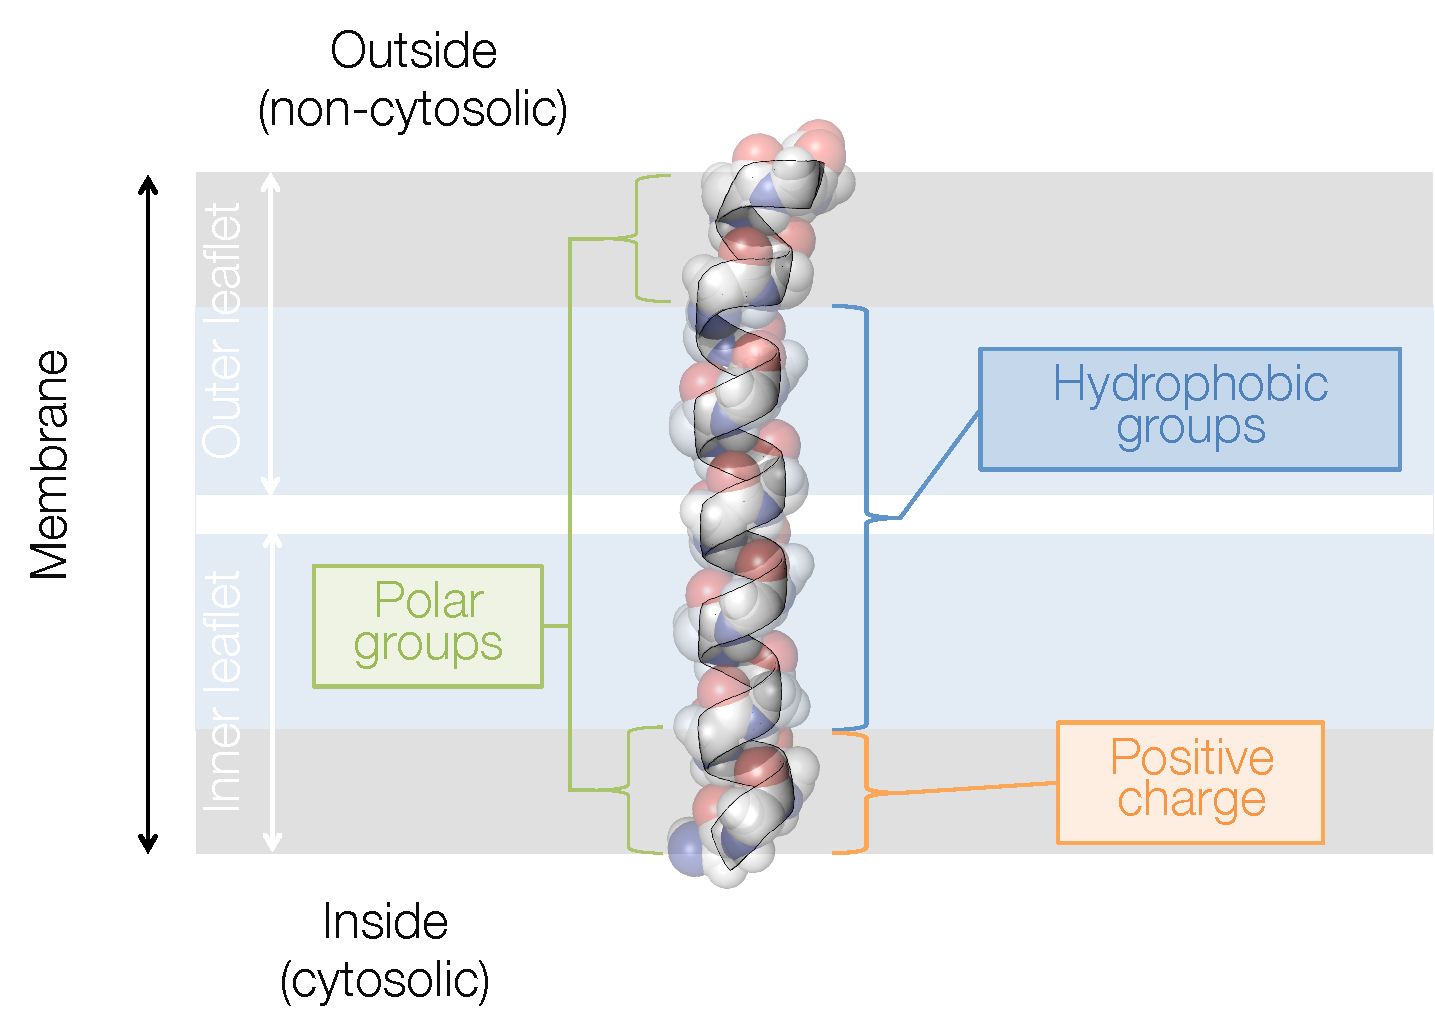
\includegraphics[width=1\textwidth]{Helix_anatomy}
\caption{A cartoon showing the general components of the membrane and a typical \gls{tmh}. The example used here for illustrative purposes is transmembrane region of tetherin (PDB 2LK9) \cite{Skasko2012}. Dark grey areas denote the area of lipid head groups. The residues in these areas are often described as flanking regions, and are often in contact with the aqueous interface of the membrane. The helix core is mostly composed of hydrophobic groups. More recently the hydrophobic group region has been associated with cell localisation and a broad range of biochemical functions \cite{Junne2010, Wong2012}. Although the regions labelled here generally hold true in terms of the statistical distribution of polar, non-polar, and charged groups, it is by no means absolute laws and many proteins break these ``rules'' \cite{Sharpe2010, Baeza-Delgado2013, Pogozheva2013}. Note that the definition of a \gls{tm} $\alpha$-helix is not entirely clear; how far the helix rises into the water-interface region to qualify as a \gls{tmh} for example \cite{VonHeijne2006}.}
\label{fig:helixcartoon1}
\end{figure}


% Figure: A cartoon depicting various problematic, yet biologically observed topologies and lengths that the alpha helices can adopt. From left to right: a typical and traditional \gls{tmh}, an exceptionally long \gls{tmh}, a \gls{tmh} that lies flat in the interface region, a kinked helix that enters and exits the bilayer on the same leaflet, a \gls{tmh} that is not long enough to span the entire membrane. Note that these exceptional formations present a challenge for topology predictions of the loop regions.}


Properties that can be analysed by bioinformatics, the sequence complexity and hydrophobicity, of the \gls{tmh} have been used to predict the role of the \gls{tmh} as either functional or structural, and as a discrete cluster from other SCOP annotated helices \cite{Wong2012}. Those findings demonstrated that the sequence of the \gls{tmh} holds valuable information regarding biological roles, and forms the basis of our interest in the link between the polarity of a helix and functional activity beyond structural anchorage.

The language used to describe \gls{tmh}s varies somewhat across the literature, primarily due to a changing understanding of \gls{tmh} general structure and relevance to function over the last 15 years or so. There is a general composition of a \gls{tmh} despite specific protein and membrane constraints \cite{Sharpe2010}.

%This paragraph should certainly be changed to the updated one from the manuscript.
A study by Baeza-Delgado {\it et al.} from 2013 \cite{Baeza-Delgado2013} looked at \gls{tmh}s in 170 integral membrane proteins from a manually maintained database of experimentally confirmed \gls{tmp}s; MPTopo \cite{Jayasinghe2001}. The group examined the distribution of residues along the \gls{tmh}s. As expected, half of the natural amino acids are equally distributed along Transmembrane (TM) helices whereas aromatic, polar, and charged amino acids along with proline are biasedly near the flanks of the TM helices \cite{Baeza-Delgado2013}. Transitions between the different types of amino acid at the ends of the hydrophobic core occur in a more defined region on the cytosolic side than at the extra cytosolic face. This is probably reflecting the different lipid composition of both leaflets of biological membranes \cite{Baeza-Delgado2013}. A larger study using 1192 human and 1119 yeast predicted \gls{tmh}s that were not structurally validated further explored the difference in \gls{tmh} and leaflet structure by exploiting the evolutionarily conserved sequence differences between the \gls{tmh} in the inner and outer leaflets \cite{Sharpe2010}. \gls{tmh}s from vertebrates and invertebrates were found to be reasonably similar compositionally. The differences in consensus \gls{tmh} structure implies that there are general differences between the membranes of the golgi and \gls{er}. The abundance of serines in the region following the lumenal end of golgi TMDs probably reflects the fact that this part of many golgi enzymes forms a flexible linker that tethers the catalytic domain to the membrane \cite{Sharpe2010}.

\subsection{The ``Positive-Inside'' rule}

Two publications by von Heijne coined the ``Positive-Inside'' rule demonstrated the practical value of positively charged residue sequence clustering in topology prediction of \gls{tmh}s in bacteria \cite{VonHeijne1989,VonHeijne1992}. It was clearly defined and shown that positively charged residues more commonly were found on the ``inside'' of the cytoplasm rather than the periplasm of {\it E. coli}. More recently still large scale sequence analysis of \gls{tmh}s from different organelle membrane surfaces in eukaryotic proteomes, show the clustering of positive charge being cytosolic \cite{Sharpe2010, Baeza-Delgado2013, Pogozheva2013}.


\subsection{Biogenesis of Transmembrane Proteins}
%Depth of secretion pathway & outline post-translational insertion

The ``inside'' was an imprecise term used to indirectly refer to the cytoplasmic space. To understand why the cytoplasm is the key part, one must recall how the membranes are thought to be synthesised.

\subsection{Measures of Hydrophobicity}

\section{Tail-anchored proteins}

Tail anchored proteins are a topologically distinct class of intracellular proteins defined by their single carboxy-terminal transmembrane domain with a cytosolic facing amino-terminus. Tail anchored proteins are involved in a range of key cellular functions including protein translocation and apoptosis. Additionally, within the tail anchored class of proteins are a set of vesicle fusion proteins called \gls{snare} proteins. There is biomedical interest in \gls{snare} drug delivery mechanisms. \gls{snare}s can fuse liposomes containing various drug payloads into the membrane. This study aims to identify \gls{snare} proteins in eukaryotic proteomes by filtering through large datasets using automatically predicted TrEMBL consensus, and manually annotated SWISS-PROT transmembrane regions. The pipeline generates a list of singlepass proteins with a transmembrane domain close to the C terminal, that are not splice isoforms. A previous study predicted 411 tail anchor proteins \cite{Kalbfleisch2007}.

Notably, known \gls{snare} transmembrane helices are highly hydrophobic even compared to other tail anchored transmembrane helices.

\section{Spontaneous membrane insertion}
%move on to case studies involving spontaneous insertion?
Signal anchored proteins, proteins that contain a single hydrophobic segment that serves as both a mitochondrial targeting signal and a membrane anchor, as well as tail anchored proteins have been shown to be able to spontaneously insert into the membrane \cite{Elisa2012, Lan2000, Colombo2009}.

It is postulated that there are electrostatic factors in the flanking regions that contribute to this spontaneous membrane insertion. Our experimental collaborators in Stephen High’s group are interested in a small group of tail anchored proteins that have very polar transmembrane domains and are capable of liposome membrane insertion without insertion machinery, also known as spontaneous insertion. They have found that chimeric synaptobrevin, one of the first identified \gls{snare} proteins, is capable of spontaneous insertion if it’s tail anchor domain is replaced by the transmembrane domains belonging to a protein of known spontaneously inserting domains. Their studies have moved the focus of spontaneous insertion away from the loop regions and onto the biophysicochemical factors of the TMH itself. The idea that \gls{snare} proteins are modular, and capable of spontaneous insertion has significant implications for both biomedical application in liposome based drug delivery and can aid future research for testing complex biological molecular networks \cite{Allen2013, Nordlund2014}.

\section{Aims of this thesis.}


\chapter{The ``negative-not-inside'' rule}
\section{Abstract}

\section{Introduction}
As the idea of positive residues inside the cytoplasm emerged during the late 1980s, so did the idea of negative residues working in concert with \gls{tmh} orientation. It was shown that removing a single lysine residue reversed the topology of a model Escherichia coli protein, whereas much higher numbers of negatively charged residues are needed to reverse topology \cite{Nilsson1990}. One would also expect to see a skew in negatively charged distribution if a cooperation between oppositely charged residues orientated a \gls{tmh}, however there is no conclusive evidence in the literature for an opposing negatively charged skew \cite{Granseth2005, Nilsson2005, Sharpe2010, Baeza-Delgado2013, Pogozheva2013}. However, in {\it E. coli} negative residues do experience electrical pulling forces when travelling through the SecYEG translocon indicating that negative charges are biologically relevant \cite{Ismail2015}.

\section{Methods}

\subsection{Normalisation}

$c_r=\frac{(a_{K,r}+a_{R,r})-(a_{D,r}+a_{E,r})}{N}$

$p_{i,r}=\frac{a_{i,r}}{\underset{r}{\max}{(a_r)}}$

$q_{i,r}=\frac{100·a_{i,r}}{a_i}$

\section{Biophysicochemical differences in multi-pass and single-pass helices}

\chapter{Tail-anchored protein discovery} %Mutants outlined + any results from Abbi
\section{Introduction}
\section{Methods}
\section{An up to date tail-anchor dataset}
\section{Potential tail-anchored SNARE protein discovery}
\section{Investigating biology of spontaneously inserting tail anchored proteins}


\chapter{The good, the bad, and the ugly helices} %Perhaps this will be for a later date!
\section{Abstract}
\section{Introduction}
\section{Methods}
\section{Results}

\chapter{Conclusions}


% This would be better at the begining so that before we get started, let's print the glossaries.
% In order for this to work a special build sequence is needed. http://tex.stackexchange.com/a/46732/42423
\printglossary[type=\acronymtype,title=Abbreviations]
\printglossary[title=Nomenclature] % Uncomment this line to use the nomenclature section.

%This line prints the bibliography ;)
%One of the references has a "-" in the wrong place and screws up the Bibliography. %the planque reference is messed up. It may need changing with every bib.tex update unless the permannet record is changed.
\printbibliography[title={Bibliography}]

% Uncomment the following THREE lines if you do have an Appendix
%\appendix
%\chapter{}
%.........

\end{document}
